\documentclass{article}
\usepackage{spconf,amsmath,graphicx}
\usepackage[hidelinks]{hyperref}
\usepackage{cleveref}

\title{Using neural network to detect native versus non-native English Speakers}

\name{Kanan Schmid, Andrew Braun, Adam Belhouchat}
\address{UCLA ECE 114 -- Speech and Image Processing. Professor F. Lorenzelli}

\begin{document}
%\ninept

\maketitle

\begin{abstract}
	In this project, we trained a neural network to differentiate between native and non-native English speakers given speech signals of the same sentence.
	We extracted MFCCs from each signal and fed them into a CNN and an RNN.
	Throughout the report, the analysis and accuracy of many different methods to compare speech will be discussed. 
	Our best results were achieved using a CNN given mean and standard deviation of MFCCs and an RNN given a time sequence of MFCCs.
\end{abstract}

\begin{keywords}
accent ID,
machine learning,
neural network
\end{keywords}

\section{Introduction}
\label{sec:intro}

A neural network is a category of artificial intelligence that uses large sets of data to train and learn such that it can take a new piece of data that it has never seen before and analyze it.
Most often, this is used to organize information into groups, such that new data can be accurately assigned to the group in which is belongs.
In this project, we used a data set of 170 speech signals, each of which is a different individual speaking the same sentence, to train a neural net to classify native versus non-native English speaker. 

The project is restricted to use only the provided data set, which is notably very small, and seemingly inaccurate in its classifications in some cases.
In other words,  some of the speakers labeled as native clearly struggle to speak the words, and have accents not associated with any English-speaking countries.
Due to these factors, the primary goal is to figure out what the most effective characteristics regarding speech are, and not necessarily to come up with a perfect identification system.
Our methodology was to try out different features or characteristics that could logically separate native and non-native English speakers.
These features could be extracted from a speech signal and fed into the neural net to differentiate between native and non-native speakers.

\section{Unsuccessful trials}
\label{sec:unsuccessful}

In this section, we will briefly describe the many different features and analyses that were ineffective or less effective than the final features.

\subsection{Speech normalization}
\label{subsec:normalization}

One of the most important hurdles in this project was ensuring that the same parts of the signals were being compared.
For example, if we compare two different signals at the 11th second, it is unlikely they will be saying the same thing at that time.
To get around this, there must be a way to  either choose features that encompass the whole signal (like pitch, which should be relatively constant throughout), or find some way to normalize the signals.
The most common way of doing this is dynamic time warping.
Dynamic time warping compares two similar signals of different duration and attempts to normalize them in the time domain.

The issue is that performing dynamic time warping on these long signals, some with over a million samples, requires extremely computationally and data intensive work.
MATLAB suggested that it needed to use matrices that were 10 TB in size.
We then tried time warping small frames of each signal, but this would distort them to the point of being unrecognizable.
Moreover, since we had more than two signals, it would be difficult to perform dynamic time warping that made them all equivalent.
We also attempted to use Euclidean distance from the training data to 3 known speakers that had non-noisy speech, different accents, and different voices (one male American, one female British, one male Irish).
Unfortunately, this feature did not correlate well and during training gave a testing error of ~52\%.

\subsection{Vowel extraction}
\label{subsec:vowel}

We also attempted to use DARLA’s vowel extraction tools \cite{DARLA} to extract formants and vowel sounds from the speech files so we would be able to easily compare vowel sounds across different accents.
However, their vowel extraction tool was not consistent enough on our dataset.
Due to the wide range in voice types and recording quality, it could not extract all vowels for each signal, even after denoising the speech files, and for some files it would completely fail to process.
Therefore we could not obtain a set of all vowels and their formants for all speech files, so we could not make use of this tool in our final network.

\subsection{Time-domain / FFT hybrid network}
\label{subsec:fft}

Another attempt at experimenting was the creation of a hybrid network in order to make the binary decision whether or not a speaker was a native speaker.
Using raw FFT / Time-Domain features yielded in low testing error (50\%, essentially guessing), as this would be a very computationally complex task to do.
The configuration of the network is given in \Cref{fig:hybrid}.

\begin{figure}[htb]
	\centering
	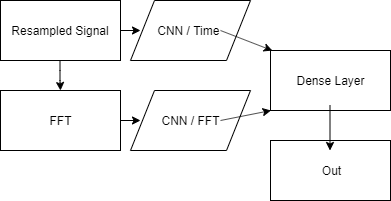
\includegraphics[width = 8.5cm]{figs/hybrid_network}
	\caption{Diagram of hybrid network.
	Various activation functions were explored in this architecture, however testing validation results were always low.}
	\label{fig:hybrid}
\end{figure}

\subsection{Filter bank energies}
\label{subsec:fbe}

Lastly, we attempted to use filter bank energies in our neural network.
Previous research has shown success using filter bank energies, or FBEs, for accent classification and speech recognition \cite{Paliwal, chuaccent}.
However, when we tested it in our implementation we did not see any improvement in testing accuracy and occasionally saw a decrease.
We attempted to use FBEs both by themselves and in addition to MFCCs, but neither attempt gave promising results.

\section{Most successful results}
\label{sec:success}

\subsection{CNN: MFCC average and standard deviation}
\label{subsec:cnn}

Our decision to use MFCCs as a feature was based off previous speech research done in the field: MFCCs have been previously used for Gaussian Mixture Models and other speech research \cite{mfccs, chuaccent}.
We believed that non-native English speakers would be more likely to have a higher variation in MFCCs across each frame.
In our implementation, the mean and standard deviation of the MFCCs over all the frames were fed into a simple feed-forward neural network and achieved testing accuracy (depending on the train / test split) anywhere from 58 - 69\%.

\begin{figure}[htb]
	\centering
	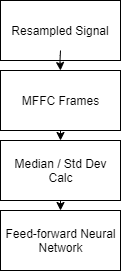
\includegraphics[width = 2.25cm]{figs/cnn_architecture}
	\caption{A diagram of the neural network architecture.}
	\label{fig:cnn_architecture}
\end{figure}

\begin{figure}[htb]
	\centering
	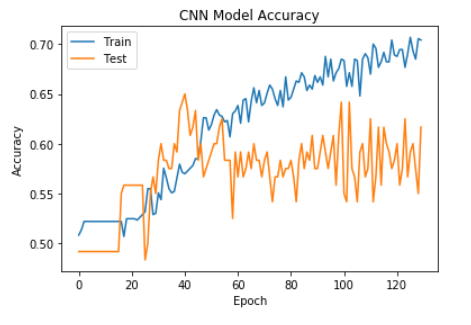
\includegraphics[width = 8.5cm]{figs/cnn_graph}
	\caption{A graph of averaged training error vs testing error over 5 different splits for the CNN implementation.}
	\label{fig:cnn_graph}
\end{figure}

The performance of this CNN was as sufficient as the LSTM / RNN implementation, however, this implementation was more susceptible to the errors in labeling and quantity of positive and negative examples of native English speakers.
Note that overfitting occurs past epoch 40, however implementation of an  l1 / l2 regularizer did not sufficiently control this overfitting.

\subsection{LSTM/RNN implementation with VoiceBox preprocessed features}
\label{subsec:rnn}

This other implementation also resulted in a validation accuracy of 68\%, but with a test accuracy of 58\%.
The features used were the features extracted from voicebox in the files “feat\_vec.mat”, which contained MFCCs for all speech signals.
For each frame of each signal, 12 MFCCs were calculated and stored in a large array.
The VoiceBox features performed poorly in a simple feed-forward neural network, but performed excellently in this network.
The performance of this is similar to the feed-forward neural network done previously.
Note that overfitting doesn’t seem to ever occur in this model, as the training accuracy seems to be bounded under 0.64.

\begin{figure}[htb]
	\centering
	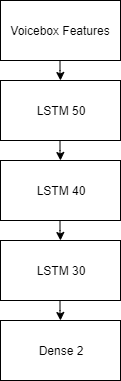
\includegraphics[width = 2.25cm]{figs/rnn_architecture}
	\caption{Architecture of the LSTM RNN implementation.}
	\label{fig:rnn_architecture}
\end{figure}

\begin{figure}[htb]
	\centering
	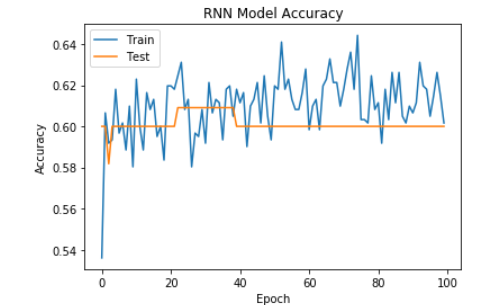
\includegraphics[width = 8.5cm]{figs/rnn_graph}
	\caption{A graph of averaged training accuracy vs testing accuracy over 5 different splits for the RNN implementation.}
	\label{fig:rnn_graph}
\end{figure}

\section{Libraries used}
\label{sec:libraries}

For this project, we tried out many different tools and libraries to extract features from our speech signals.

\texttt{VoiceBox}: We used VoiceBox to generate features such as sF0 - sF4, Energy, SHR on different frames of the speech signal, MFCCs, filter bank energies, and LPCs.
The features from VoiceBox performed poorly in a  feedforward neural network but performed well in the RNN architecture.

\texttt{VoiceSauce}: We experimented with the formants, pitch, and B1-B4 features from Praat as well as H1, H2, and H4, A1, A2, and A3, cepstral peak prominence, and harmonic-to-noise ratio.
However, none of these gave better performance than the VoiceBox features.

\texttt{fastdtw}: Calculation of overall Euclidean distance of one speech signal to another.
Created distance features that were experimented with, but unfortunately, did not perform well enough as stated in \Cref{subsec:normalization}.

\texttt{python\_speech\_features}: Used to create MFCC features (averages and standard deviations) that were used in our best-performing CNN.

\texttt{DARLA}: Vowel extraction tool from Dartmouth.
Performs automatic and semi-automatic vowel extraction given a speech signal, a transcript of what was said in the signal, and some characteristics of the speaker.
Unfortunately, the tool performed too inconsistently for it to be useful in our project.

\section{Future work}
\label{sec:future}

Overall, the models could have been significantly improved with more data.
It was observed that our data had “noisy-labelling”, where some people claimed to be English speakers but spoke slowly and with a non-English accent.
Additionally, our dataset is rather small, meaning that more complex architectures would be impossible with our data size.
In the future, I would add significantly more data (thousands or tens of thousands of speakers) in order to test these models, which would reduce the impact of noisy labelling and allow for the exploration of more complex architectures.

\section{Conclusion}
\label{sec:conclusion}

Overall, it seems that the RNN had more consistent performance than our CNN implementation.
However, the CNN implementation significantly reduced complexity and was able to run more than 100 epochs in less than a minute, whereas the RNN architecture required an hour to run 100 epochs.
We’ve demonstrated two architectures that can be used to achieve 60\% testing accuracy on the dataset.

\bibliographystyle{IEEEbib}
\bibliography{refs}

\end{document}
